% !Mode::"TeX:UTF-8"

% -------------------- Information --------------------

\newcommand{\TITLE}{补充题四}
\newcommand{\AUTHOR}{Jason}
\newcommand{\SUBJECT}{复变函数补充题}

% -------------------- Packages --------------------

\documentclass[a4paper,12pt]{ctexart}
\usepackage{amsmath}
%\usepackage{amsthm} % 定理格式 由ntheorem代替.
\usepackage{amssymb}
\usepackage{authblk} % 作者 (见校赛论文).
\usepackage{array}
\usepackage{bigfoot} % to allow verbatim in footnote.
\usepackage{boldline} % 长表格表格线加粗.
\usepackage{caption} % 题注.
\usepackage{commath} % abs, norm
\usepackage{enumerate}
%\usepackage{enumitem} 用enumerate包代替.
\usepackage{fancyhdr} % 脚注.
\usepackage{filecontents}
\usepackage{flafter} % 不让float出现在定义之前的地方.
\usepackage{float} % 你们这帮float给我乖乖听话 HHHHHHHHHHH.
\usepackage[T1]{fontenc} % Bera Mono Font
\usepackage{fontspec} % 字体.
\usepackage{graphicx}
\usepackage{hyperref}
\usepackage{lastpage}
\usepackage{listings} % 排版程序语言.
\usepackage{longtable} % 长表格.
\usepackage{makecell} % 表格线加粗 \Xhline{1.2pt}.
\usepackage{mathtools} % \xleftrightarrow.
\usepackage{multirow} % 合并单元格.
\usepackage[square, numbers, sort&compress]{natbib} % 引用.
\usepackage[thmmarks, amsmath, thref]{ntheorem} % 定理格式.
\usepackage[section]{placeins} % 使图像不会显示在别的部分 若过于严格则换成[below].
\usepackage{stackrel} % 上下写 见校赛论文.
\usepackage{subcaption} % subcaption and subfigure
\usepackage{SUBSubsubsection}
\usepackage{titlesec} % Section标题格式.
\usepackage{varioref} % For Cross References.
\usepackage[dvipsnames]{xcolor} % 颜色声明.
\usepackage[all,cmtip]{xy} % Commutive diagram.

% Require `ntheorem'

\usepackage{DefaultTheoremStyle}
\usepackage[mathlines, edtable]{lineno} % Line numbers.
    %\begin{edtable}{tabular}[<args>] <entries> \end{edtable}

% Require `xcolor'

\usepackage[numbered, framed]{matlab-prettifier}
\usepackage{pgfplots}
\usepackage{tikz}

% Incompatible with `matlab-prettifier'

\usepackage[printwatermark]{xwatermark} % Foreground Watermarks.

% -------------------- Settings --------------------

\title{\TITLE}
\author{\AUTHOR}
\date{\today}

% Package: caption

\captionsetup{
    margin    =   6pt,
    font      =   small,
    labelfont =   bf
}

% Package: ctex

\setCJKfamilyfont{fzstk}{FZShuTi} % 方正舒体
\newcommand{\fzstk}{\CJKfamily{fzstk}}

% Package: fancyhdr

\setlength{\headheight}{15pt}
\lhead{Copyright \copyright\ \AUTHOR}
\rhead{Page \thepage\ of \pageref{LastPage}}

% Package: graphicx

\graphicspath{{resources/}} %图像文件目录
    
% Package: hyperref

\hypersetup{
    linktoc             =   all,
    colorlinks          =   true,
    linkcolor           =   TealBlue,
   %anchorcolor         =   Black,
    citecolor           =   Blue,
   %filecolor           =   Cyan,
   %menucolor           =   Red,
   %runcolor            =   filecolor,
    urlcolor            =   magenta,
    pdfinfo             =   {
        Title           =   {\TITLE},
        Author          =   {\AUTHOR},
        Subject         =   {\SUBJECT}},
    bookmarksnumbered   =   true,
    pdfstartview        =   FitH,
    pdfpagelayout       =   OneColumn
}

% Package: lineno

\renewcommand{\linenumberfont}{\normalfont\scriptsize\sffamily}

\let\oldlstinputlisting\lstinputlisting
\renewcommand{\lstinputlisting}[2][\empty]{
    \par\nolinenumbers\oldlstinputlisting[#1]{#2}\linenumbers\par
}

\let\oldlstlisting\lstlisting
\let\oldendlstlisting\endlstlisting
\renewenvironment{lstlisting}
    {\par\nolinenumbers\oldlstlisting}
    {\oldendlstlisting\endnolinenumbers\par}

\let\oldtable\table
\let\oldendtable\endtable
\renewenvironment{table}
    {\par\nolinenumbers\oldtable}
    {\oldendtable\endnolinenumbers\par}

% Package: listings

\lstMakeShortInline[style=MATLAB-editor, basicstyle=\mlttfamily]|

\lstset{
    breaklines=true,
    backgroundcolor=\color{lightgray},
    basicstyle=\scriptsize,
    numbers=left,
    numberstyle={\color{black!33}\scriptsize\sffamily},
    xleftmargin=2em,
    xrightmargin=2em
}

% Package: pgfplot

\pgfplotsset{width=7cm, compat=1.16}

% Package: varioref

\renewcommand{\reftextbefore}
    {on the \reftextvario{preceding page}{page before}}
\renewcommand{\reftextafter}
    {on the \reftextvario{following}{next} page}
\renewcommand{\reftextfacebefore}
    {on the \reftextvario{facing}{preceding} page}
\renewcommand{\reftextfaceafter}
    {on the \reftextvario{facing}{next}{page}}
\renewcommand{\reftextfaraway}[1]
    {on page \pageref{#1}}

% Package: xwatermark

\newsavebox\mybox
\savebox\mybox{\tikz[color=cyan, opacity=0.2]\node{\fzstk\SUBJECT};}
\newwatermark*[
    allpages,
    angle=45,
    scale=6,
    xpos=-20,
    ypos=15
]{\usebox\mybox}

% -------------------- General new commands --------------------

\DeclareMathAlphabet{\mathsfsl}{OT1}{cmss}{m}{sl}

\DeclareMathOperator{\diff}{d}

\newcommand{\matr}[1]{\ensuremath{\mathsfsl{#1}}} % italic sans serif
\newcommand{\me}{\mathrm{e}}
\newcommand{\mi}{\mathrm{i}}
\newcommand{\restrict[1]}{\raisebox{-.5ex}{$|$}_{#1}}

% -------------------- Specific new commands --------------------

\DeclareMathOperator{\arcosh}{arcosh}
\DeclareMathOperator{\Arcosh}{Arcosh}
\DeclareMathOperator{\Log}{Log}

% -------------------- Document --------------------

\begin{document}

    % -------------------- Title Page --------------------

    \maketitle
    \thispagestyle{empty}
    \pagenumbering{roman}

    % -------------------- Abstract Page --------------------

    % -------------------- Contents --------------------

    %\newpage
    %\tableofcontents

    % -------------------- Body --------------------

    \newpage
    \pagestyle{fancy}
    \pagenumbering{arabic}
    \linenumbers
    
    \begin{problem}
        设$\sqrt[3]{4z-3}$的某个单值分支$w(z)$满足$w(2)>0$, 请用三种方式割破复平面
        使得该分支的$w(i)$恰好分别取得所有三个值.
    \end{problem}

    \begin{solution}
        见如下三张图.
        \begin{figure}[H]
            \begin{subfigure}{.49\textwidth}
                \centering
                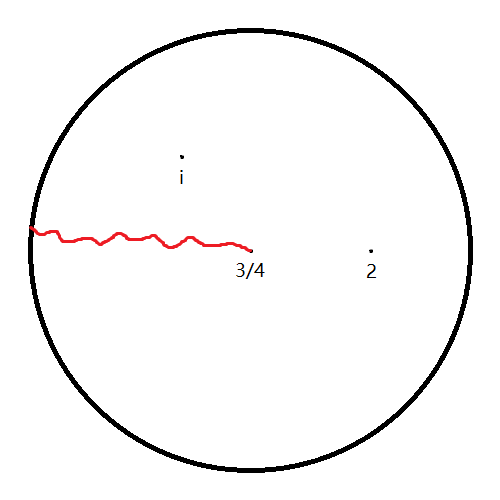
\includegraphics[scale=0.5]{0.png}
                \caption{$\displaystyle w(i)=\sqrt[3]{5}\me^{\arg(-3+4\mi)/3}$}
                \label{figure_0}
            \end{subfigure}   
            \begin{subfigure}{.49\textwidth}
                \centering
                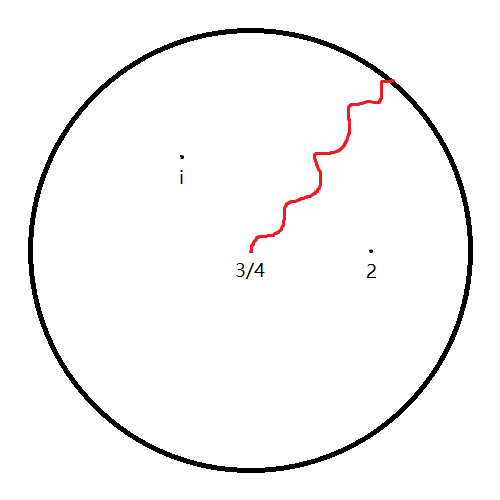
\includegraphics[scale=0.5]{-2pi.png}
                \caption{$\displaystyle w(i)=
                    \sqrt[3]{5}\me^{(\arg(-3+4\mi)-2\pi)/3}$}
                \label{figure_-2pi}
            \end{subfigure}
            \caption{两张直着切的}
            \label{figure_straight}
        \end{figure}
        \begin{figure}[H]
            \centering
            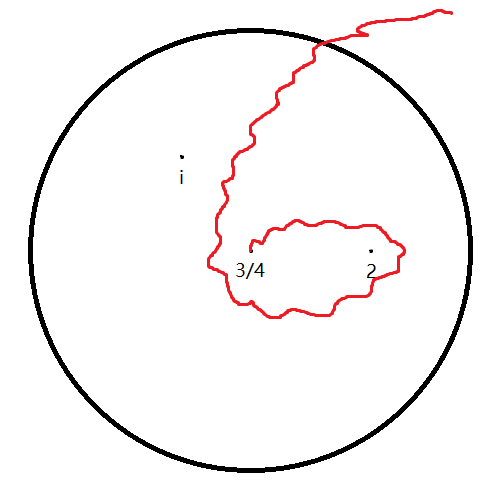
\includegraphics[scale=0.5]{-4pi.png}
            \caption{$\displaystyle w(i)=\sqrt[3]{5}
                \me^{(\arg(-3+4\mi)-4\pi)/3}$}
            \label{figure_-4pi}
        \end{figure}
        即为所求分割方式.
    \end{solution}

    \begin{problem}
        回顾平面积分的Green公式.
        记$\displaystyle\omega=\frac{x\diff y-y\diff x}{x^2+y^2}$,
        则$\diff \omega=0$.
        但是$\omega$在原点有奇性,
        因此积分$\displaystyle\int_{1}^{z}{\omega}$与路径有关, 进而
        $\displaystyle f(z)=\int_{1}^{z}{\omega}$是$\mathbb{C}_{*}$
        上的一个多值函数.
        \begin{enumerate}[(1)]
            \item 求出$f(z)$的所有值, 即各种路径积分的值.
            \item 将$\omega$表示为$z, \bar{z}, \diff z, \diff \bar{z}$的形式,
                证明: $\partial\omega=0, \bar{\partial}\omega=0$.\\
                {[}若$\omega=f\diff z+g\diff \bar{z}$, 则
                $\partial\omega:=\partial f\wedge\diff z
                    +\partial g\wedge\diff \bar{z},
                \bar{\partial}\omega:=\bar{\partial} f\wedge\diff z
                    +\bar{\partial} g\wedge\diff \bar{z}${]}
        \end{enumerate}
    \end{problem}

    \begin{solution}
        我们知道
        \begin{equation}
            \int_{\mathbb{S}^{1+}}{\omega} = 2\pi,
        \end{equation}
        所以
        \begin{equation}
            f(z) = \{2k\pi, k\in\mathbb{Z}\}.
        \end{equation}

        由于$\displaystyle x=\frac{z+\bar{z}}{2}, y=\frac{z-\bar{z}}{2\mi}$,
        有
        \begin{equation}
            \omega = \frac{1}{2\mi}(\frac{\diff z}{z}+
            \frac{\diff \bar{z}}{\bar{z}}). 
        \end{equation}
        于是$f=1/(2\mi z), g=1/(2\mi\bar{z})$.
        故
        \begin{equation}
            \partial\omega=\partial f\wedge\diff z
                +\partial g\wedge\diff \bar{z}
            =
            \frac{\partial g}{\partial z}\diff z\wedge\diff \bar{z}
            =
            0,
        \end{equation}
        且
        \begin{equation}
            \bar{\partial}\omega=\bar{\partial} f\wedge\diff z
                +\bar{\partial} g\wedge\diff \bar{z}
            =
            \frac{\partial f}{\partial \bar{z}}\diff \bar{z}\wedge\diff z
            =
            0.
        \end{equation}
    \end{solution}

    \begin{problem}
        在复球面意义下, 请分别画出$w_{1}=\sqrt{z(z-1)(z-2)}$和
        $w_{2}=\sqrt{z(z-1)(z-2)(z-3)}$
        的黎曼面的草图.
    \end{problem}

    \begin{solution}
        草图如下.
        \begin{figure}[H]
            \begin{subfigure}{.49\textwidth}
                \centering
                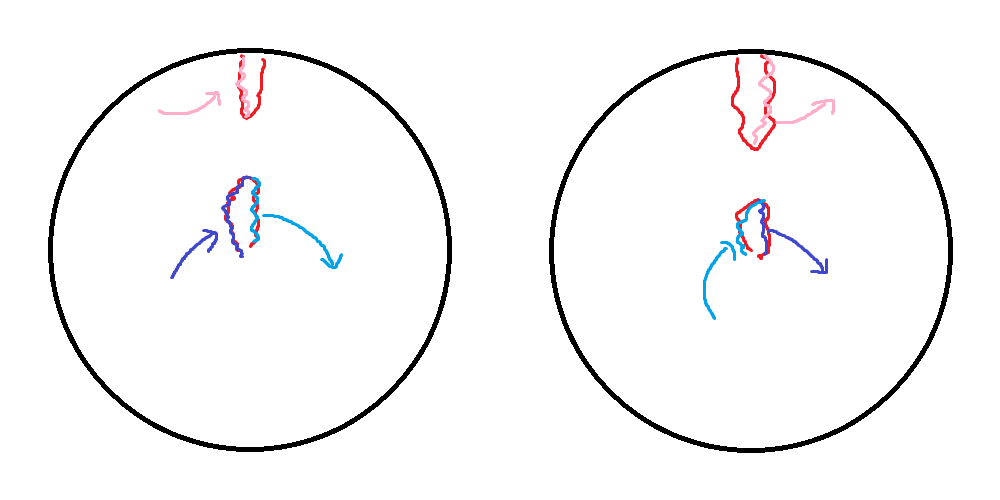
\includegraphics[scale=0.25]{riemann_3.png}
                \caption{$w_{1}=\sqrt{z(z-1)(z-2)}$}
                \label{figure_riemann_3}
            \end{subfigure}   
            \begin{subfigure}{.49\textwidth}
                \centering
                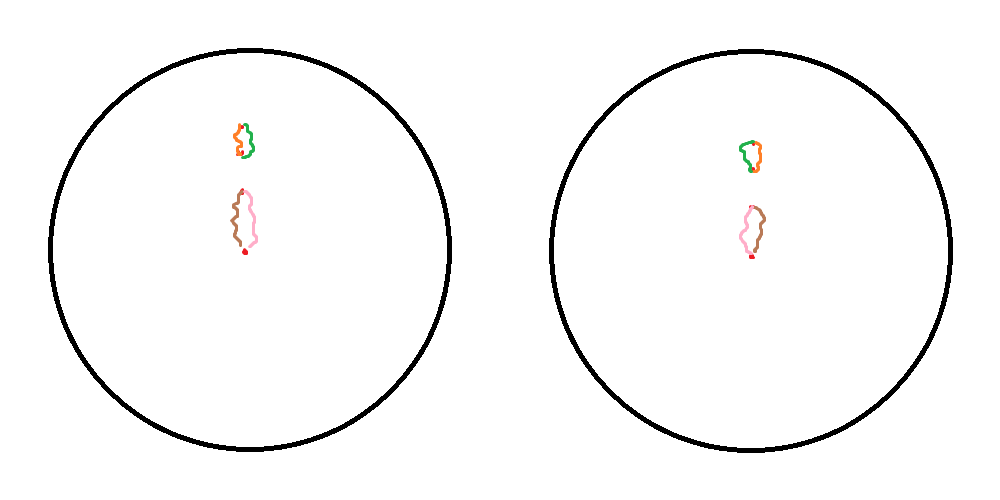
\includegraphics[scale=0.25]{riemann_4.png}
                \caption{$w_{2}=\sqrt{z(z-1)(z-2)(z-3)}$}
                \label{figure_riemann_4}
            \end{subfigure}
            \caption{黎曼面草图}
            \label{figure_riemann}
        \end{figure}
    \end{solution}

    \begin{problem}
        请适当割破复平面, 得到$w=\Arcosh(z)$的单值解析分支.
    \end{problem}

    \begin{solution}
        通过计算, 有
        \begin{equation}
            \begin{aligned}
                z &= \cosh{w}\\
                z &= \frac{\me^{w}+\me^{-w}}{2}\\
                \me^{w} &= z+\sqrt{z^{2}-1}\\
                w &= \Log{(z+\sqrt{z^{2}-1})}
            \end{aligned}
        \end{equation}
        于是若我们沿着线段$[-1,1]$割破复平面,
        就能得到$\sqrt{z^{2}-1}$的单值解析分支.

        再考虑$z+\sqrt{z^{2}-1}$的值域, 如果在该值域内可良定$\log$函数,
        那么就大功告成了.
    \end{solution}

    % -------------------- Bibliography --------------------

    %\newpage
    %\bibliography{Principles_of_Mathematical_Analysis}
    %\bibliographystyle{plain}

\end{document}
